\documentclass[12pt]{article}
\usepackage{amscd,amssymb,amsthm,amsxtra,exscale,latexsym,verbatim,paralist}
\usepackage{mathrsfs}
\usepackage[T1]{fontenc}
\usepackage{newtxmath,newtxtext}
\usepackage[margin=1in]{geometry}

%\usepackage{mathtools}
%\usepackage{multicol}
\usepackage{tikz}

\pagestyle{empty} 
\setlength{\parindent}{0pt} 
\setlength{\parskip}{\baselineskip}

\theoremstyle{plain}
\newtheorem{ex}{Exercise}

\renewcommand{\proofname}{Solution}

%\makeatletter
%\renewcommand*\env@matrix[1][*\c@MaxMatrixCols c]{%
%  \hskip -\arraycolsep
%  \let\@ifnextchar\new@ifnextchar
%  \array{#1}}
%\makeatother

\begin{document}

MTH 385 \qquad Homework due 2022-03-07

\begin{ex} [3.5.1]
  Explain the solution $x=21/4$, $y=71/8$ to $x^3-3x^2+3x+1=y^2$ given by Diophantus (Heath~(1910), p. 242) by constructing the tangent through the obvious rational point on this curve (Figure~3.4).
\end{ex}

\begin{center}
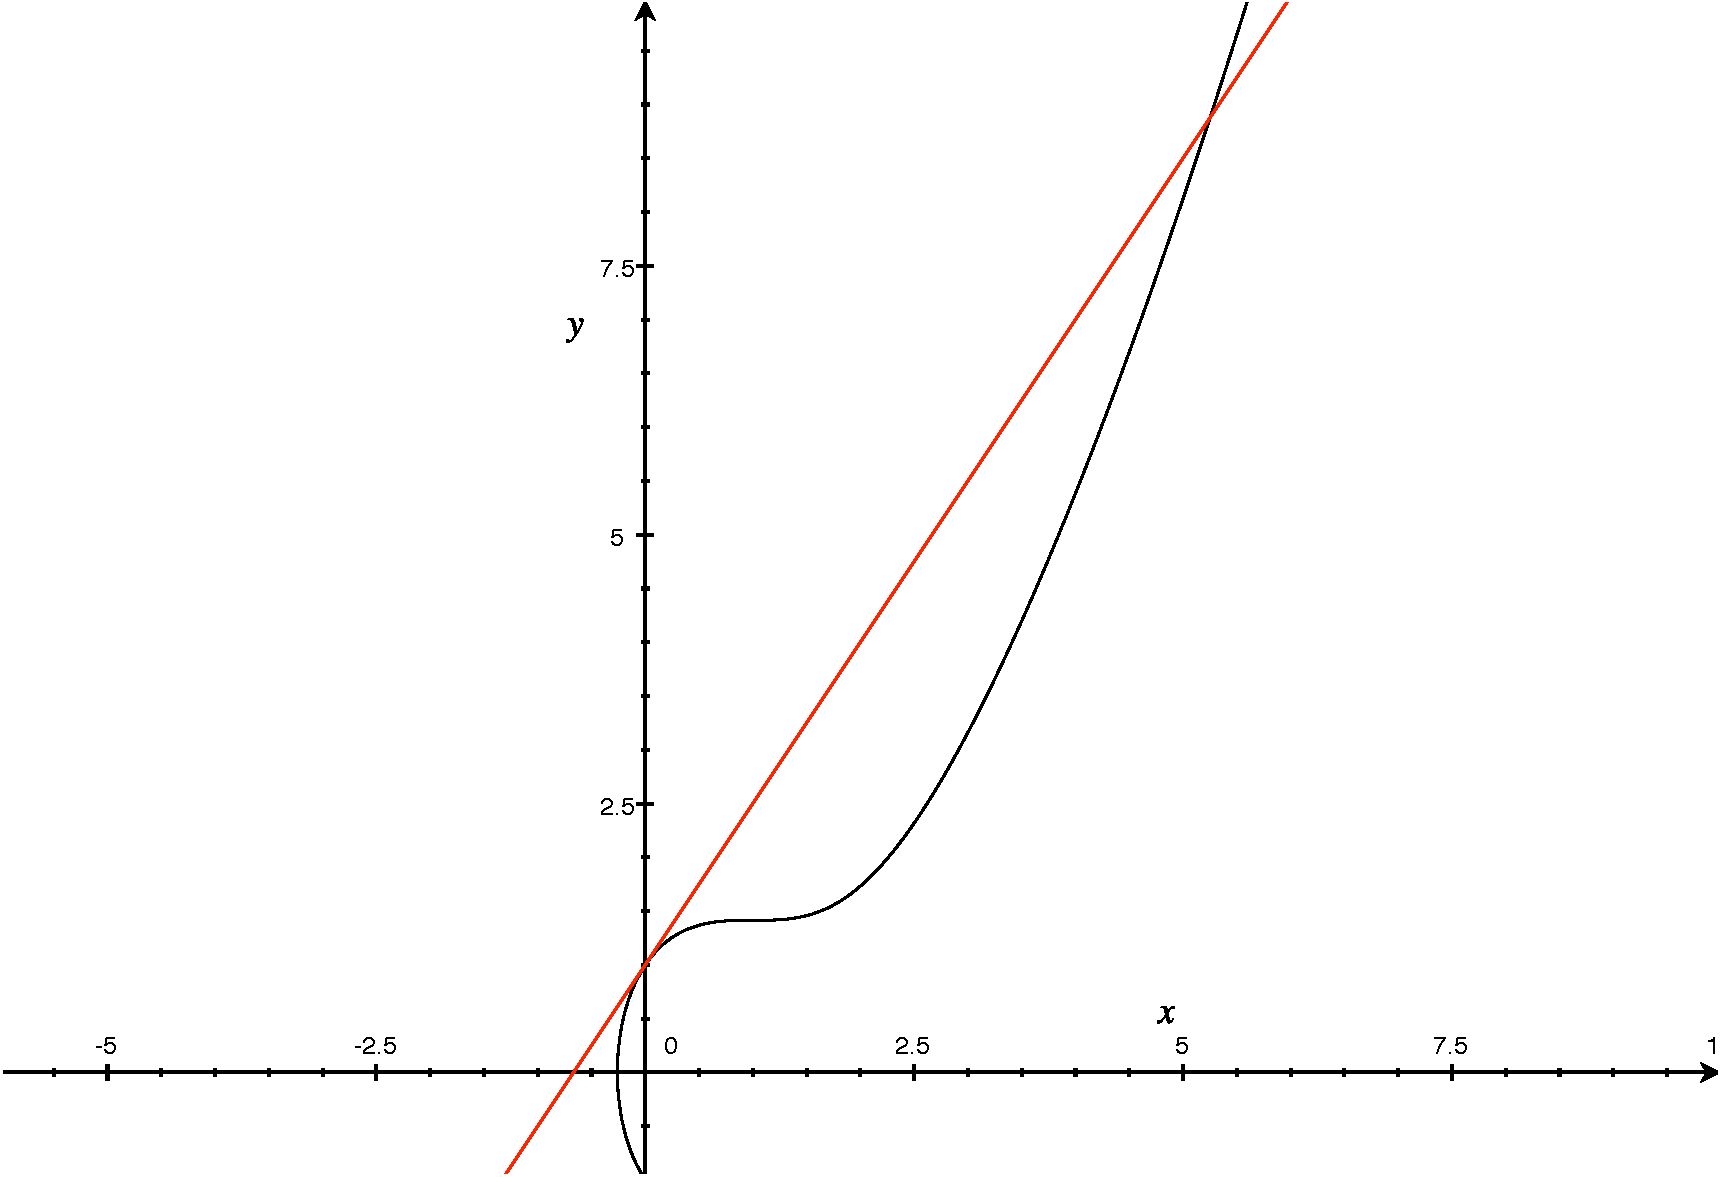
\includegraphics[scale=0.5]{cubic}

Figure~3.4: Cubic curve $y^2=x^3-3x^2+3x+1$ and tangent
\end{center}

\begin{proof}
  The obvious rational point is $(0,1)$. Use implicit differentiation to compute the slope of the tangent line.
  \begin{align*}
    3x^2-6x+3                         &= 2y\frac{dy}{dx} \\
    3\cdot0^2-6\cdot0+3               &= 2\cdot1\cdot\frac{dy}{dx}\Bigg|_{\substack{x=0 \\ y=1}} \\
    \frac{dy}{dx}\Bigg|_{\substack{x=0 \\ y=1}} &= \frac{3}{2}
  \end{align*}
  So, the point-slope and slope-intercept form of the equation of the tangent line are
  \[
    y=\frac{3}{2}(x-0)+1\text{ and }y=\frac{3}{2}x+1.
  \]
  Now, we make the substitution $y=\frac{3}{2}x+1$ in the equation for the curve. The zeroes of this equation are the $x$-coordinates of the intersection points of the curve and the tangent line.
  \begin{align*}
    x^3-3x^2+3x+1                   &= \left(\frac{3}{2}x+1\right)^2 \\
    x^3-3x^2+3x+1                   &= \frac{9}{4}x^2+3x+1 \\
    x^3-\frac{21}{4}x^2             &= 0 \\
    x^2\left(x-\frac{21}{4}\right)  &= 0
  \end{align*}
  \emph{This polynomial is divisible by $x^2$ because the line is tangent to the curve at the point $(0,1)$.} Now, we find the $y$-coordinate of the point on the tangent line whose $x$-coordinate is $\frac{21}{4}$.
  \[
    y=\frac{3}{2}\cdot\frac{21}{4}+1=\frac{71}{8}
  \]
\end{proof}

\begin{ex} [3.5.2]
  Rederive the following rational point construction of Vi\`{e}te~(1593), p. 145. Given the rational point $(a,b)$ on $x^3-y^3=a^3-b^3$ , show that the tangent at $(a,b)$ is
  \[
    y=\frac{a^2}{b^2}(x-a)+b
  \]
  and that the other intersection of the tangent with the curve is the rational point
  \[
    x=a\frac{a^3-2b^3}{a^3+b^3},\qquad y=b\frac{b^3-2a^3}{a^3+b^3}.
  \]
\end{ex}

\begin{proof}
  Use implicit differentiation to compute the slope of the tangent line.
  \begin{align*}
    3x^2-3y^2\frac{dy}{dx}              &= 0 \\
    3a^2-3b^2\frac{dy}{dx}\Bigg|_{\substack{x=a \\ y=b}}  &= 0 \\
    \frac{dy}{dx}\Bigg|_{\substack{x=a \\ y=b}}           &= \frac{a^2}{b^2}
  \end{align*}
  So, the point-slope form of the equation of the tangent line is
  \[
    y=\frac{a^2}{b^2}(x-a)+b.
  \]
  Now, we make the substitution $y=\frac{a^2}{b^2}(x-a)+b$ in the equation for the curve. The zeroes of this equation are the $x$-coordinates of the intersection points of the curve and the tangent line.
  \begin{align*}
    x^3-\left(\frac{a^2}{b^2}(x-a)+b\right)^3                                       &= a^3-b^3 \\
    x^3-\left(\frac{a^2}{b^2}(x-a)+b\right)^3-a^3+b^3                               &= 0 \\
    x^3-a^3-\frac{a^6}{b^6}(x-a)^3-3\frac{a^4}{b^3}(x-a)^2-3a^2(x-a)-b^3+b^3        &= 0 \\
    (x-a)(x^2+ax+a^2)-\frac{a^6}{b^6}(x-a)^3-3\frac{a^4}{b^3}(x-a)^2-3a^2(x-a)      &= 0 \\
    (x-a)\left(x^2+ax+a^2-\frac{a^6}{b^6}(x-a)^2-3\frac{a^4}{b^3}(x-a)-3a^2\right)  &= 0 \\
    (x-a)\left(x^2+ax-2a^2-\frac{a^6}{b^6}(x-a)^2-3\frac{a^4}{b^3}(x-a)\right)      &= 0 \\
    (x-a)\left((x-a)(x+2a)-\frac{a^6}{b^6}(x-a)^2-3\frac{a^4}{b^3}(x-a)\right)      &= 0 \\
    (x-a)^2\left(x+2a-\frac{a^6}{b^6}(x-a)-3\frac{a^4}{b^3}\right)                  &= 0
  \end{align*}

  \emph{Notice two things: (1) the cubic polynomial we obtain is divisible by $(x-a)^2$ because the line is tangent to the (original) cubic curve at the point $(a,b)$; (2) this calculation might have been simplified by making the substitution $x=w+a$ to get $(w+a)^3-\left(\frac{a^2}{b^2}w+b\right)^3=a^3-b^3$ because the resultant cubic polynomial would be divisible by $w^2$.}

  \begin{align*}
    x+2a-\frac{a^6}{b^6}(x-a)-3\frac{a^4}{b^3}                                      &= 0 \\
    \frac{b^6-a^6}{b^6}x                                                            &= \frac{3a^4b^3-a^7-2ab^6}{b^6} \\
    \frac{b^6-a^6}{b^6}x                                                            &= a\frac{3a^3b^3-a^6-2b^6}{b^6} \\
    x                                                                               &= a\frac{3a^3b^3-a^6-2b^6}{b^6-a^6} \\
                                                                                    &= a\frac{3a^3b^3-a^6-2b^6}{(b^3-a^3)(b^3+a^3)} \\
                                                                                    &= a\frac{-(a^3-b^3)(a^3-2b^3)}{-(a^3-b^3)(a^3+b^3)} \\
                                                                                    &= a\frac{a^3-2b^3}{a^3+b^3}
  \end{align*}
  Now, we find the $y$-coordinate of the point on the tangent line whose $x$-coordinate is $a\frac{a^3-2b^3}{a^3+b^3}$.
  \begin{align*}
    y &= \frac{a^2}{b^2}\left(a\frac{a^3-2b^3}{a^3+b^3}-a\right)+b \\
      &= \frac{1}{a^3+b^3}\left(\frac{a^3}{b^2}(a^3-2b^3-a^3-b^3)+a^3b+b^4\right) \\
      &= \frac{1}{a^3+b^3}(-3a^3b+a^3b+b^4) \\
      &= b\frac{b^3-2a^3}{a^3+b^3}
  \end{align*}
\end{proof}

The \emph{Jade Mirror of Four Unknowns} does not go beyond four equations in four unknowns (hence the name). The idea is quite general, but it becomes hard to implement on the counting board when there are more than four unknowns. An amusing problem in three unknowns from the \emph{Jade Mirror}, which does not require the full strength of the elimination method, is given in the exercises below.

\begin{ex} [5.2.4]
  Problem~2 in the Jade Mirror (see Hoe~(1977), p. 135) is to find the side $a$ of a right-angled triangle $(a,b,c)$ such that
  \begin{align*}
    a^2-(b+c-a) &= ab, \\
    b^2+(a+c-b) &= bc.
  \end{align*}
  The \emph{Jade Mirror} suggests choosing the unknowns $x=a$ and $y=b+c$. Using $a^2=c^2-b^2$, show that this implies
  \begin{align*}
    b &= (y-x^2/y)/2, \\
    c &= (y+x^2/y)/2.
  \end{align*}
\end{ex}

\begin{proof}
  Make the substitutions $a=x$ and $c=y-b$ in the equation $a^2=c^2-b^2$.
  \begin{align*}
    x^2 &= (y-b)^2-b^2 \\
        &= y^2-2by+b^2-b^2 \\
        &= y^2-2by \\
    2by &= y^2-x^2 \\
    b   &= (y-x^2/y)/2 \\
    \\
    c   &= y-b \\
    b   &= y-(y-x^2/y)/2 \\
        &= (2y-y+x^2/y)/2 \\
        &= (y+x^2/y)/2
  \end{align*}
\end{proof}

\begin{ex} [5.2.5]
  Deduce that the first two equations in Exercise~5.2.4 are equivalent, respectively, to
  \begin{align*}
    (-2-x)y^2+(2x+2x^2)y+x^3  &= 0 \\
    (2-x)y^2+2xy+x^3          &= 0.
  \end{align*}
\end{ex}

\begin{proof}
  Make the substitutions $a=x$, $b=(y-x^2/y)/2$ and $c=(y+x^2/y)/2$ in the equations.
  \begin{align*}
    x^2-\left(\frac{y^2-x^2}{2y}+\frac{y^2+x^2}{2y}-x\right)                                &= x\cdot\frac{y^2-x^2}{2y} \\
    2x^2y-2y^2+2xy                                                                          &= xy^2-x^3 \\
    (-2-x)y^2+(2x+2x^2)y+x^3                                                                &= 0 \\
    \\
    \left(\frac{y^2-x^2}{2y}\right)^2+\left(x+\frac{y^2+x^2}{2y}-\frac{y^2-x^2}{2y}\right)  &= \frac{y^2-x^2}{2y}\cdot\frac{y^2+x^2}{2y} \\
    \frac{y^4-2x^2y^2+x^4+4xy^2+2y^3+2x^2y-2y^3+2x^2y-y^4+x^4}{4y^2}                        &= 0 \\
    \frac{-2x^2y^2+2x^4+4xy^2+4x^2y}{4y^2}                                                  &= 0 \\
    \frac{x}{2y^2}(-xy^2+x^3+2y^2+2xy)                                                      &= 0 \\
    \intertext{We may assume $x=a>0$.}
    -xy^2+x^3+2y^2+2xy                                                                      &= 0 \\
    (2-x)y^2+2xy+x^3                                                                        &= 0
  \end{align*}
\end{proof}

\begin{ex} [5.2.6]
  By subtracting one equation in Exercise~5.2.5 from the other, deduce that $y=x^2/2$. Substitute this back to obtain a quadratic equation for $x$, with solution $x=a=4$. What are the values of $b$ and $c$?
\end{ex}

\begin{proof}
  Subtract the first equation from the second.
  \begin{align*}
    (2-x)y^2+2xy+x^3-((-2-x)y^2+(2x+2x^2)y+x^3)                         &= 0 \\
    2y^2-xy^2+2xy+x^3+2y^2+xy^2-2xy-2x^2y-x^3                           &= 0 \\
    4y^2-2x^2y                                                          &= 0 \\
    2y(2y-x^2)                                                          &= 0 \\
    \intertext{We may assume $y=b+c>0$.}
    2y-x^2                                                              &= 0 \\
    y                                                                   &= x^2/2 \\
    \\
    (2-x)\left(\frac{x^2}{2}\right)^2+2x\left(\frac{x^2}{2}\right)+x^3  &= 0 \\
    2x^4-x^5+4x^3+4x^3                                                  &= 0 \\
    -x^3(x+2)(x-4)                                                      &= 0
  \end{align*}
  We may assume $x=a>0$. So, $x=a=4$. Therefore, $y=4^2/2=8$, $b=(8-4^2/8)/2=3$, and $c=(8+4^2/8)/2=5$.
\end{proof}

\end{document}

